% \section{Hydrological model with fractures}
\subsection{Motivation for heterogeneous model}
The HM model with homogeneous rock parameters, described in Chapter \ref{ch:model_comparison}, was used to estimate the pressure in the newly drilled boreholes in the vicinity of test chambers ZK5-1J and ZK5-1S.
Comparing the results with the outcomes of the pore pressure measurements by \cite{tz_monitoring}, it turned out that the model did not explain sufficiently the measured pressure in the borehole cells.
In particular, for most of the borehole cells the model overestimated the initial value prior to excavation, and did not match the size and even the direction of pressure jumps at excavation times.
In Fig. \ref{fig:two_cells_pressure}, this mismatch is visible on two selected cells.
\begin{figure}
\centering
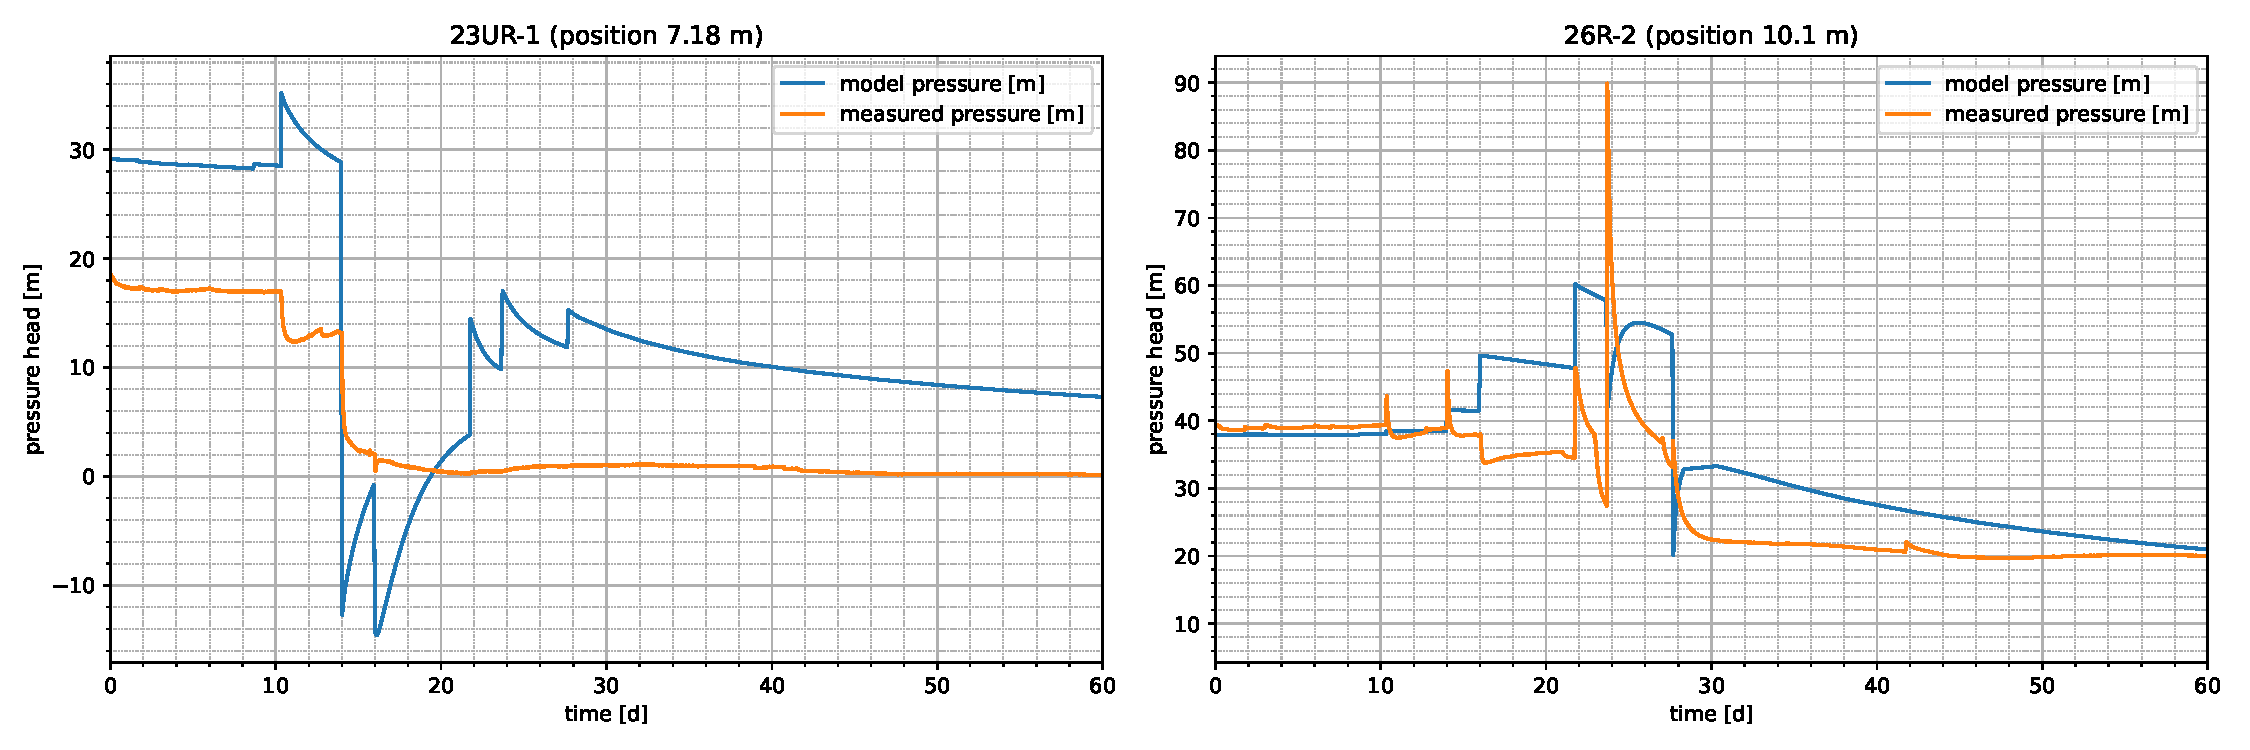
\includegraphics[width=\textwidth]{graphics/fractures/chamber_pressures_refined_compared_select}
\caption{Comparison of homogeneous model and measurement: pressure in borehole cells L5-23UR-1 and L5-26R-2 during 60 days from the beginning of excavation.}
\label{fig:two_cells_pressure}
\end{figure}
The above-mentioned differences indicate the presence of strong heterogeneities in the surrounding rock, in agreement with geological mapping and borehole-logging data.
Low observed pressure can be explained by fault zones and conductive fractures that connect the particular location with L5 laboratory gallery.
It is therefore evident that fractures and inhomogeneities need to be incorporated into the model to describe the HM response of the rock mass accurately.

The first step towards heterogeneous HM model was to identify fractures that explain the low initial pressure.
In the following subsections we describe the steps to determine the fracture geometry and physical parameters.

\subsection{Geometry of fractures}
% How we select significant fracture planes - borehole and gallery mappings.
In \cite{tz_monitoring}, detailed results of well log measurements in 8 newly drilled boreholes were presented.
Besides a large number of filled inhomogeneities, 22 open inhomogeneities with nonzero thickness were reported, see Tab. \ref{tab:well_log}.
From these, 15 items were left after removing similarly located and oriented ones, see also Fig. \ref{fig:vrty-pukliny}. 
% \sts{[Standa: Tabulka \ref{tab:well_log} a obrazek \ref{fig:vrty-pukliny} by byly uzitecne uz v Sekci 5.1, protoze pomoci nich se daji snaze interpretovat nektere vystupy ze Sekce 5.1.]}

\begin{table}
\caption{Open fractures and inhomogeneities detected by borehole logging (types of inhomogeneity: 0=damaged zone, 1=very significant, 2=significant, 3=less significant).
Gray lines were not taken into account due to their similar position and orientation to adjacent items.}
\label{tab:well_log}
\newcommand{\gr}{\color{gray}}
\begin{tabular}{@{}ccSSSSc@{}}
Id & Borehole & {Position [\unit\meter]} & {Azimuth [\unit\degree]} & {Inclination [\unit\degree]} & {Width [\unit{\milli\meter}]} & Type\\
\hline
\gr 1 & L5-49DL & \gr 2.42 & \gr 314.31 & \gr 79.52 & \gr 6.03 & \gr 1\\
2 & & 2.44 & 318.68 & 74.56 & 16.08 & 1\\
\gr 3 & & \gr 3.02 & \gr 310.23 & \gr 85.08 & \gr 10.98 & \gr 1\\
4 & & 3.07 & 127.47 & 62.18 & 8.83 & 1\\
5 & & 6.67 & 258.04 & 68.83 & 18.89 & 1\\
\hline
6 & L5-50UL & 10.85 & 301.8 & 89.56 & 29.84 & 1\\
7 & & 11.29 & 250.35 & 38.05 & 21.5 & 1\\
\hline
8 & L5-22DR & 2.96 & 230.24 & 47.43 & 39.87 & 1\\
\gr 9 & & \gr 3.41 & \gr 233.47 & \gr 58.09 & \gr 35.42 & \gr 1\\
 \hline
& L5-23UR\\
\hline
10 & L5-24DR & 0.6 & 343.38 & 65.17 & 17.37 & 1\\
11 & & 10.05 & 338.47 & 48.82 & 31.7 & 2\\
\hline
12 & L5-26R & 0.68 & 18.06 & 78.6 & 22.58 & 1\\
13 & & 2.73 & 218.01 & 49.37 & 14.57 & 3\\
\hline
14 & L5-37R & 5.25 & 200.31 & 49.51 & 47.21 & 3\\
15 & & 7.71 & 203.91 & 81.86 & 302.93 & 0\\
16 & & 10.55 & 234.23 & 62.77 & 81.39 & 2\\
17 & & 11.44 & 338.31 & 78.97 & 53.09 & 1\\
\hline
\gr 18 & L5-37UR & \gr 5.97 & \gr 235.45 & \gr 57.71 & \gr 4.63 & \gr 2\\
\gr 19 & & \gr 6.02 & \gr 239.26 & \gr 66.26 & \gr 2.74 & \gr 2\\
20 & & 6.17 & 234.68 & 46.67 & 32.64 & 1\\
\gr 21 & & \gr 6.24 & \gr 229.86 & \gr 56.21 & \gr 32.73 & \gr 1\\
\gr 22 & & \gr 6.36 & \gr 223.77 & \gr 49.46 & \gr 5.66 & \gr 2\\
\end{tabular}
\end{table}

\begin{figure}
\centering
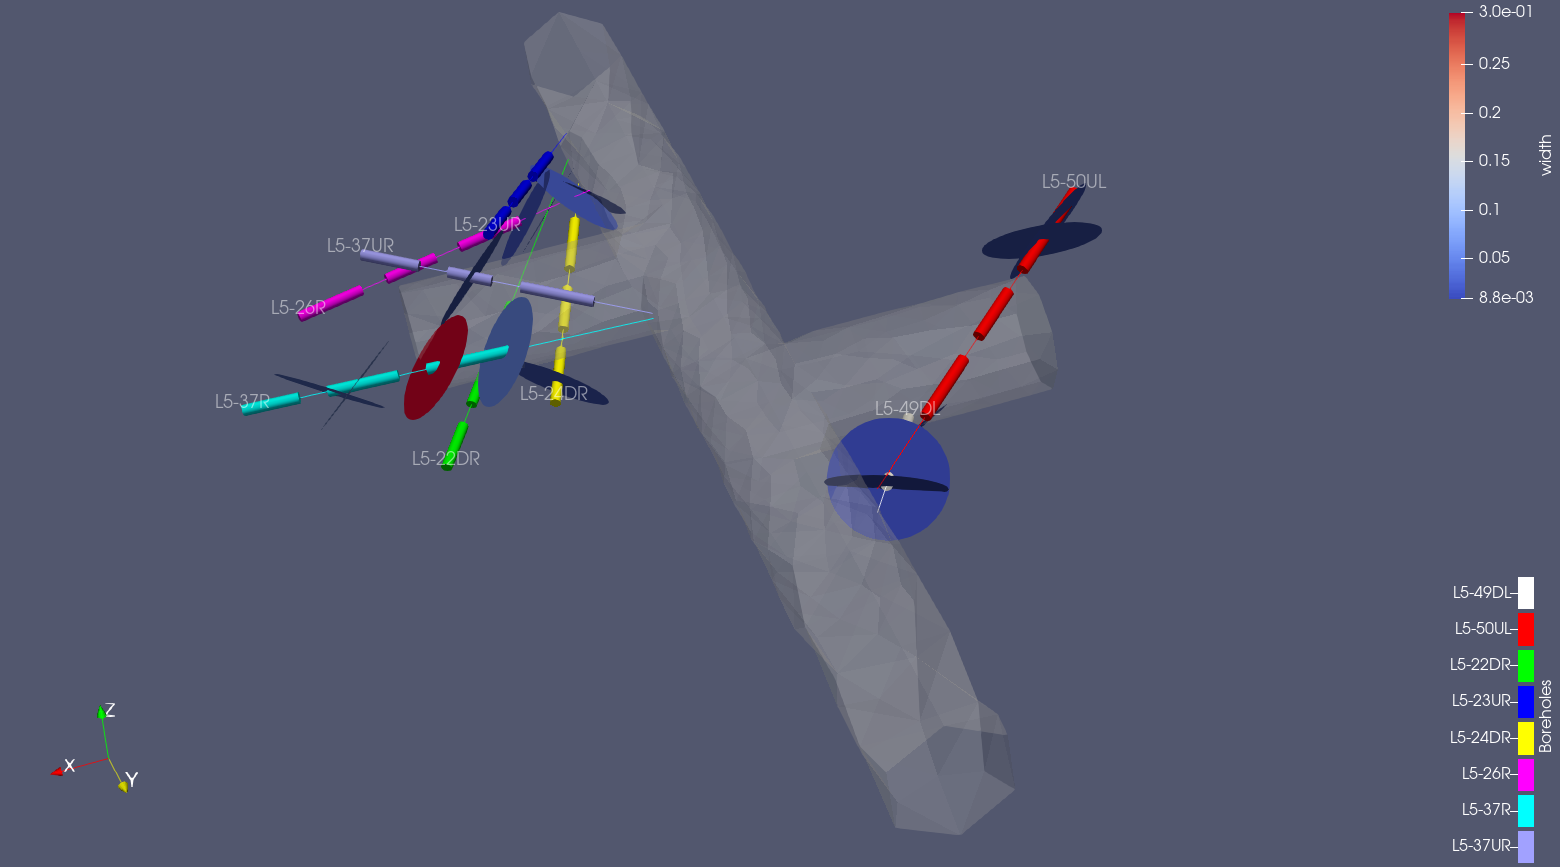
\includegraphics[width=\textwidth]{graphics/fractures/vrty-pukliny}
\caption{Boreholes and detected conductive fractures.}
\label{fig:vrty-pukliny}
\end{figure}

% Algorithm for fitting planes to prescribed points on line objects (boreholes, L5 gallery).
These data were used to heuristically determine several fracture planes that might potentially connect particular boreholes and L5 gallery.
The fracture planes were found by an automated fitting procedure to match prescribed orientation and crossing points in particular boreholes.
By this approach, we identified three fractures that could possibly connect multiple boreholes with L5 gallery:

\begin{tabular}{cc}
Fracture plane & Crossing inhomogeneities (see Tab. \ref{tab:well_log})\\
\hline
1 & 15\\
2 & 17\\
3 & 16, 20
\end{tabular}
% fr1: id 15 % pridat k fr3
% fr2: id 17 % 2?
% fr3: id 16, 20 % (8), 13

It should be noted, however, that this choice is subject to significant uncertainty and requires further revision.

% Algorithm for division of plane into regions around objects.
Since the hydraulic conductivity and aperture of fractures may vary with position, the three fracture planes were further divided into regions according to the distance to boreholes and L5 gallery, where the physical parameters are assumed constant.
This division was applied to the computational mesh, see Fig. \ref{fig:fracture_regions}.
\begin{figure}
\centering
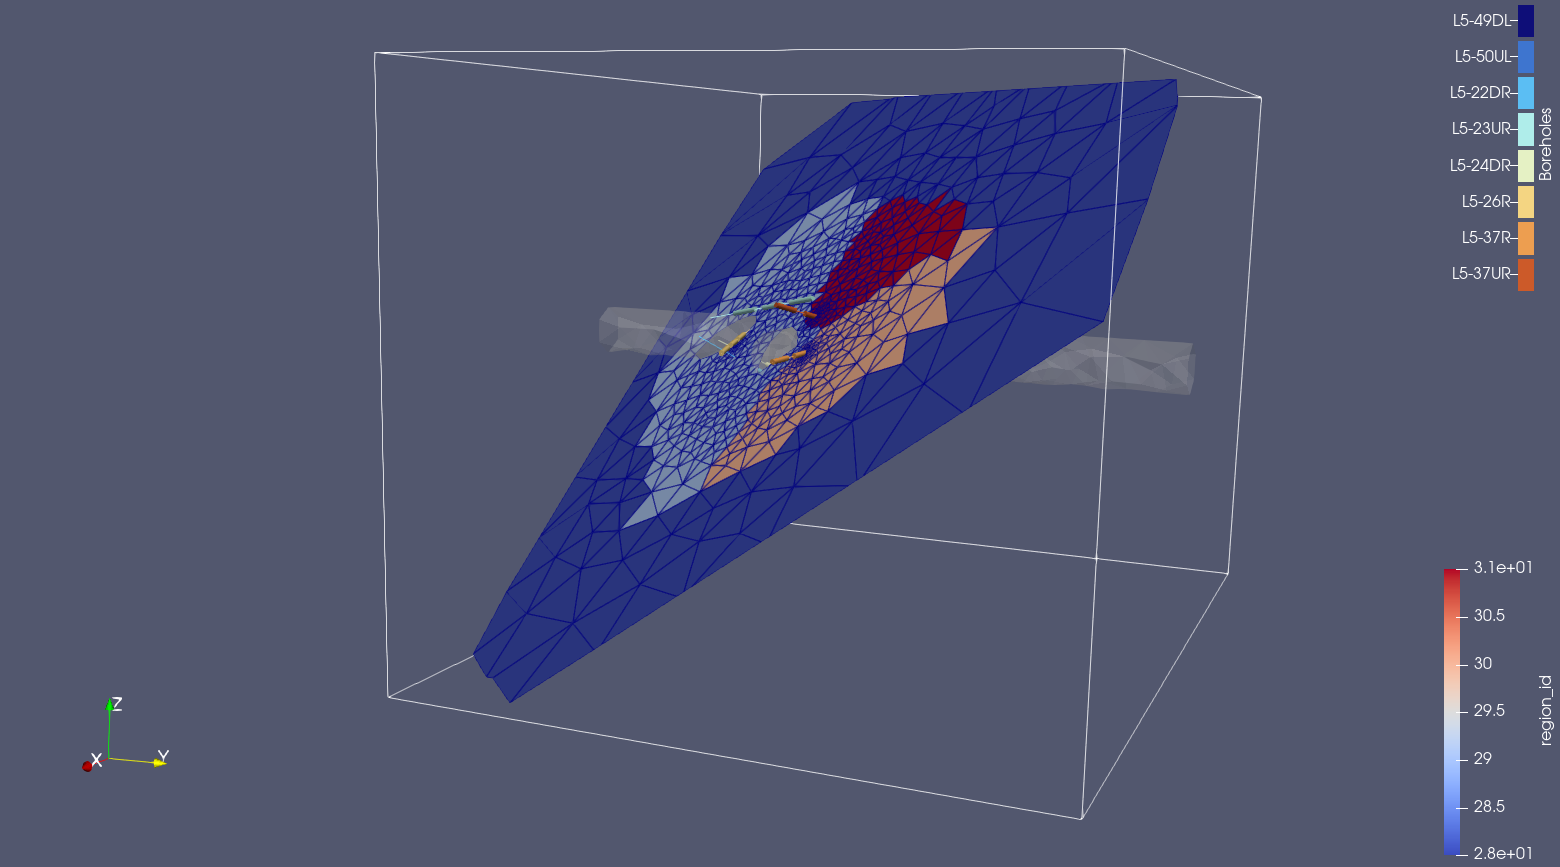
\includegraphics[width=\textwidth]{graphics/fractures/frac-regions}
\caption{Partitioning of fracture plane 3 into regions.}
\label{fig:fracture_regions}
\end{figure}


\subsection{Fitting of initial pressure}
The extended geometry of the HM model was used in a fitting procedure to match the initial pressure in borehole cells.
Based on the pore pressure measurements reported by \cite{tz_monitoring}, initial values of pressure head prior to the excavation of the test chambers were determined (Fig. \ref{fig:pressure_summary}, label \textquote{2024 manual}), later referred to as \textquote{target pressure values}.
The fracture cross-section was fixed per region using the data from well log, and the hydraulic conductivity in 11 fracture regions was calibrated to minimize the cost function
\[ f(\vc p) = \frac12\|\vc p-\vc p_{target}\|^2. \]
Here $\vc p$ is the vector of computed pressure heads and $\vc p_{target}$ is the vector of target (observed) pressure heads in 15 borehole cells (excluding boreholes L5-49DL, L5-50UL and L5-22DR). 
We used the function \verb|least_squares| from the Python library \verb|SciPy| to perform the minimization.
The computation led to a reduction of the cost function from $5411$ to $512$, i.e., to approximately $9~\%$ of the value for the original model without fractures.
The original and optimized pressure values are depicted in Fig. \ref{fig:optim_pressure}.
\begin{figure}
\centering
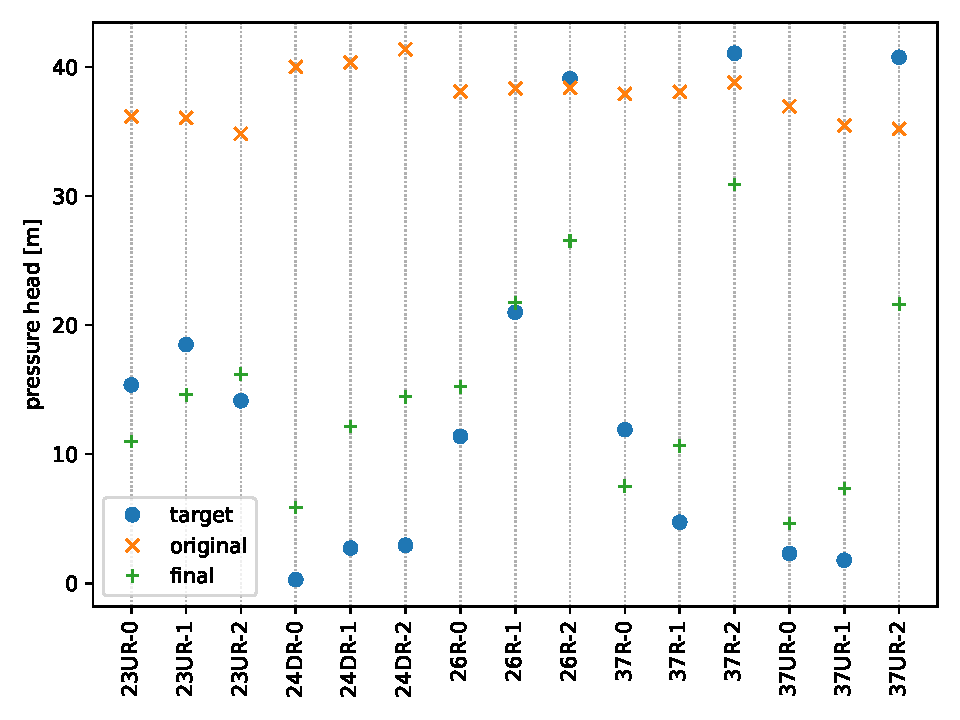
\includegraphics[width=\textwidth]{graphics/fractures/pressures}
\caption{Pressure head in borehole cells: comparison of model with homogeneous parameters (original) and optimized model with fractures (final).}
\label{fig:optim_pressure}
\end{figure}
From the figure, one can see that for most of the borehole cells, the model with three fractures yields closer values to the target ones than the model without fractures.
The result is, however, still not satisfactory.
In particular, high observed pressure in the farthest cells of L5-26R, L5-37R and L5-37UR was not matched, since the borehole cells are possibly located in isolated low-conductive regions.

\subsection{Summary}
The homogeneous HM model systematically overestimated pore pressures measured in borehole cells, which is consistent with geological evidence of strong structural heterogeneity. To improve the model, three explicit fracture planes were introduced based on the borehole logging data and geological mapping of the excavation walls. The fractures were subdivided into regions with spatially constant hydraulic properties.

Hydraulic conductivities in the fracture regions were optimized to fit observed initial pressure heads, leading to a substantial reduction of the pressure misfit to about $9~\%$ of the homogeneous model value. Although the heterogeneous model improved the agreement for most borehole cells, high pressures in several distant cells were not reproduced, indicating the likely presence of hydraulically isolated zones not captured by the current model.


% \begin{thebibliography}{9}
% \bibitem{sgg_karotaz} D. Hanák. Bukov PVP II – pórové tlaky – karotáž, zpráva o karotážním měření 8 průzkumných vrtů. SG Geotechnika, 2024.
% \bibitem{tz_porove_tlaky_1} K. Sosna. MONITORING PÓROVÝCH TLAKŮ VODY V PVP BUKOV II - PRŮBĚŽNÁ ZPRÁVA Č. 1. Technical report No. 795/2024 (SÚRAO).
% \end{thebibliography}


% \end{document}
